\tikzset{
	nodes around center/.style args={#1:#2:#3:#4}{
		at={([shift={(#3)}] {{(\tikzchaincount-1)*360/(#2)+#1}}:{#4})}
	},
	nodes around center*/.style args={#1:#2:#3:#4}{
		at={([shift={(#3.{(\tikzchaincount-1)*360/(#2)+#1})}] {{(\tikzchaincount-1)*360/(#2)+#1}}:{#4})},
		anchor={(\tikzchaincount-1)*360/(#2)+#1+180}
	}
}

\section{Auflösbare Gruppen}

\subsection{Definition} Sei $G$ eine Gruppe. Für $a,b \in G$ nennt man $[a,b]:=aba^{-1}b^{-1}$ den Kommutator\index{Kommutator} von $a$ und $b$. Man nennt $G':=\langle\{[a,b]\mid a,b\in G\}\rangle\leq G$ die Kommutatorgruppe\index{Kommutatorgruppe} von $G$. Weiter definiert man für
jedes $n\in\N_0$ die $n$-te Kommutatorgruppe $G^{(n)}$ von $G$ rekursiv durch $G^{(0)}:=G$ und $G^{(n+1)}:=(G^{(n)})'$ für $n\in\N_0$.

\subsection{Bemerkung} Sei $G$ eine Gruppe.
\begin{enumerate}[label=(\alph*)]
	\item
		$\forall a,b\in G:([a,b]=1\iff ab=ba)$
		
	\item
		$G'=\{[a_1,b_1]\cdots[a_m,b_m]\mid m\in\N_0,~a_i,b_i\in G\}$

		["`$\supseteq$"' klar; "`$\subseteq$"' beachte $[a,b]^{-1}=(aba^{-1}b^{-1})^{-1}=bab^{-1}a^{-1}=[b,a]$ für $a,b\in G$]
		
	\item
		$G'$ ist der kleinste Normalteiler $N$ von $G$ mit $G/N$ abelsch.

		[$G'$ ist nach \ref{fixed:1.3.12} eine charakteristische Untergruppe und daher ein Normalteiler von $G$; ist $N \normsub G$ mit $G/N$ abelsch, so $\bar{[a,b]}^N=\bar a \bar b \bar a^{-1} \bar b^{-1}=\bar{aa^{-1}}^N \bar{bb^{-1}}^N=1$ und daher $[a,b]\in N$ für alle $a,b\in G$, woraus $G'\subseteq N$ folgt.]
\end{enumerate}

\subsection{Definition} Sei $n\in\N_0$. Eine Permutation der Form
$$	(x_1,...,x_\ell):=
	\left(
		\begin{array}{l}
			\{1,...,n\} \to \{1,...,n\} \\
			\begin{tikzpicture}
			  \node (Z) {};
			  \begin{scope}[
			    start chain=circle placed {nodes around center=270:6:Z:3em},
			    every join/.append style={<-|},
			    every node/.append style={
			      on chain=circle,
			      join,
			      minimum size=2em
			      }
			  ]
			    \foreach \cnt in {4,...,1}
			      \node {$x_\cnt$};
			          \node {$x_\ell$};
			    \node[rotate=130] {\dots};
			    \chainin (circle-begin);
			  \end{scope}
			\end{tikzpicture}\\
			x \mapsto x \text{ für } x \in \{1,...,n \} \setminus \{x_1,...,x_\ell\}
		\end{array}
	\right)
$$
mit $\ell\in\{2,...,n\}$ und paarweise verschiedenen $x_1,...,x_\ell\in\{1,\dots,n\}$ nennt man einen $\ell$-Zykel\index{Zykel@$\ell$-Zykel} in $S_n$. Man nennt $2$-Zykel auch Transpositionen \LAref{9.1.3}.

\subsection{Proposition} \ALref{\ref{fixed:1.1.12}} Sei $n\in\N_0$. Dann
$$A_n=\{\sigma_1\cdots\sigma_m\mid m\in\N_0,~\sigma_1,\dots,\sigma_m\text{ $3$-Zykel in }S_n\}.$$

\proof "`$\supseteq$"': Seien $x_1,x_2,x_3\in\{1,...,n\}$ paarweise verschieden. Zu zeigen: $(x_1\ x_2\ x_3)\in A_n$. Dies folgt aus $(x_1\ x_2\ x_3)=(x_2\ x_3)(x_1\ x_3)$.

"`$\subseteq$"': Sind $x_1,x_2,x_3,x_4\in\{1,...,n\}$ paarweise verschieden, so
$(x_1\ x_2)(x_3\ x_4)=(x_1\ x_3\ x_2)(x_1\ x_3\ x_4)$. Sind $x_1,x_2,x_3\in\{1,\dots,n\}$ paarweise verschieden, so $(x_1\ x_2)(x_2\ x_3)=(x_1\ x_2\ x_3)$. Sind $x_1,x_2\in\{1,\dots,n\}$ mit $x_1\ne x_2$, so $(x_1\ x_2)(x_1\ x_2)=1$. \qed

\subsection{Proposition} Sei $n\in\N_0$. Dann $S_n'=A_n$ und
$$
A_n'=
\begin{cases}
	\{1\}&\text{falls $n\le 3$,}\\
	V_4:=\{1,(1\ 2)(3\ 4),(1\ 3)(2\ 4),(1\ 4)(2\ 3)\}\cong V&\text{falls $n=4$,}\\
	A_n&\text{falls $n\ge5$.}
\end{cases}
$$
\begin{figure}[h]
	\centering
	\tikzstyle{every node} = [align=center]
	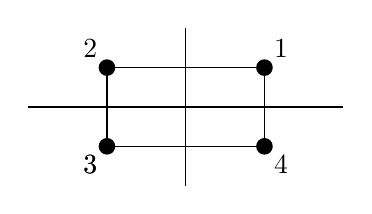
\begin{tikzpicture}[baseline=1.1em]
		\coordinate (a) at (0,0);
		\coordinate (b) at (2,0);
		\coordinate (c) at (2,1);
		\coordinate (d) at (0,1);
		\draw (a) -- (b) -- (c) -- (d) -- (a);
		\fill (a) circle (3pt);
		\fill (b) circle (3pt);
		\fill (c) circle (3pt);
		\fill (d) circle (3pt);
		\node[below left] at (0,0) {3};
		\node[below left] at (0,0) {3};
		\node[above left] at (0,1) {2};
		\node[above right] at (2,1) {1};
		\node[below right] at (2,0) {4};
		\draw (-1,0.5) -- (3,0.5);
		\draw (1,-0.5) -- (1,1.5);
	\end{tikzpicture} \quad {\ALref{\ref{fixed:1.1.9e}}}
\end{figure}

\proof ~

\underline{$S_n'\subseteq A_n$:} Nach \ref{fixed:3.3.2c} genügt es zu zeigen, dass $S_n/A_n$ abelsch ist. Dies ist klar, da $S_n/A_n \eqtilde C_2$ für $n\ge2$ \ref{fixed:1.3.18} und $S_n/A_n \eqtilde C_1$ für $n\in\{0,1\}$.

\underline{$A_n\subseteq S_n'$:} Nach \ref{fixed:3.3.4} genügt es zu zeigen, dass jeder $3$-Zykel in $S_n'$ liegt. Seien hierzu $x_1,x_2,x_3$ paarweise verschieden. Dann
$$(x_1\ x_2\ x_3)=(x_1\ x_3)(x_2\ x_3)(x_1\ x_3)^{-1}(x_2\ x_3)^{-1}=[(x_1\ x_3),(x_2\ x_3)]\in S_n'.$$


\underline{$A_n'=\{1\}$ für $n\le3$:} Für $n\le3$ ist $A_n \eqtilde A_n/\{1\}$ abelsch, da $\#A_n\le\#A_3=\frac{\#S_3}2=\frac{3!}2=3$.

\underline{$A_4'=V_4$:} "`$\subseteq$:"' Wegen $\#A_4=\frac{4!}2=4\cdot3=12$ gilt
$\#(A_4/V_4)=3$ und $A_4/V_4$ ist abelsch.

"`$\supseteq$:"' Ist $\{x_1,x_2,x_3,x_4\}=\{1,2,3,4\}$, so nach \ref{fixed:3.3.4}
\begin{align*}
	(x_1\ x_2)(x_3\ x_4)&=(x_1\ x_2\ x_3)(x_1\ x_2\ x_4)(x_1\ x_2\ x_3)^{-1}(x_1\ x_2 x_4)^{-1}\\
	&=[\underbrace{(x_1\ x_2\ x_3)}_{\in A_4},\underbrace{(x_1\ x_2\ x_3)}_{\in A_4}]\in A_4'.
\end{align*}

\underline{$A_n'=A_n$ falls $n\ge5$:} Sei $n\ge5$. Zu zeigen: $A_n\subseteq A_n'$. Seien $x_1,x_2,x_3\in\{1,...,n\}$ paarweise verschieden. Zu zeigen: $(x_1\ x_2\ x_3)\in A_n'$. Wähle $x_4,x_5\in\{1,...,n\}\setminus\{x_1,x_2,x_3\}$ mit $x_4\ne x_5$. Dann
$$
	(x_1\ x_2\ x_3)
	=(x_1\ x_2\ x_4)(x_1\ x_3\ x_5)(x_1\ x_2\ x_4)^{-1}(x_1\ x_3\ x_5)^{-1}
	=[(x_1\ x_2\ x_4),(x_1\ x_3\ x_5)]\in A_n'.
$$ \qed

\subsection{Definition} Sei $G$ eine Gruppe. Es heißt $(G_0,...,G_n)$ eine Normalreihe\index{Normalreihe} von $G$, wenn $G=G_0\normsup G_1\normsup...\normsup G_n=\{1\}$. In diesem Fall heißen die Gruppen $G_k/G_{k+1}$ ($k\in\{0,... n-1\}$) die Faktoren\index{Faktor!einer Normalreihe} dieser Normalreihe. Es heißt $G$ auflösbar\index{auflösbar}, wenn $G$ eine Normalreihe mit (lauter) abelschen Faktoren besitzt.

\subsection{Satz} Sei $G$ eine Gruppe. Dann
$$\text{$G$ auflösbar}\iff\exists n\in\N_0:G^{(n)}=\{1\}.$$

\proof "`$\Longleftarrow$"' Ist $n\in\N_0$ mit $G^{(n)}=\{1\}$, so ist $(G^{(0)},...,G^{(n)})$ eine Normalreihe von $G$ mit abelschen Faktoren.

"`$\implies$"' Sei $(G_0,...,G_n)$ eine Normalreihe von $G$ mit abelschen Faktoren. Wir zeigen durch Induktion nach $k\in\{0,...,n\}$, dass $G^{(k)}\subseteq G_k$:

\underline{$k=0$:} $G^{(0)}=G=G_0$

\underline{$k\to k+1$ \quad ($k\in\{0,...,n-1\}$)} \quad $G^{(k+1)}=(G^{(k)})' \overset{\text{IV}}{\underset{G^{(k)}\subseteq G_k}\subseteq} G_k'
\overset{\substack{G_k/G_{k+1} \\ \text{abelsch}}}\subseteq G_{k+1}$ \qed

\subsection{Satz} $S_n$ ist auflösbar für $n\le4$, nicht aber für $n\ge5$.

\proof Nach Proposition \ref{fixed:3.3.5} gilt $S_n^{(2)}=A_n'=\{1\}$ für $n\le3$,
$$S_4^{(3)}=A_4^{(2)}=V_4'\overset{\substack{V_4 \eqtilde V \eqtilde C_2\times C_2\\ \text{abelsch}}}=\{1\}$$
und $S_n^{(1)}=S_n^{(2)}=...=A_n\ne\{1\}$ für $n\ge5$. \qed

\subsection{Proposition} Sei $G$ eine Gruppe.
\begin{enumerate}[label=(\alph*)]
	\item
		Ist $G$ auflösbar und $H\le G$, so ist auch $H$ auflösbar.
		
	\item
		Ist $N \normsub G$, so
		$$\text{$G$ auflösbar}\iff(\text{$N$ auflösbar} \text{ \& } \text{$G/N$ auflösbar}).$$
\end{enumerate}

\proof ~

\textbf{zu (a):} Klar, da man durch Induktion $H^{(n)}\subseteq G^{(n)}$ für alle $n\in\N_0$ zeigt.

\textbf{zu (b):} Gelte $N \normsub G$. Durch Induktion zeigt man $(G/N)^{(n)}=(G^{(n)}N)/N$ für alle $n\in\N_0$ \ref{fixed:1.4.1}:

\underline{$n=0$:} $G/N=\underbrace{(GN)}_{=G}/N$

\underline{$n\to n+1$ ($n\in\N_0$):}
\begin{eqnarray*}
	(G/N)^{(n+1)}&=&((G/N)^{(n)})'\overset{\text{IV}}=((G^{(n)}N)/N)'\\
	&\overset{\text{\ref{fixed:3.3.2b}}}=&\{[\bar{a_1n_1}^N,\bar{a_1'n_1'}^N]\dotsm[\bar{a_mn_m}^N,\bar{a_m'n_m'}^N]
	\mid m\in\N_0,~a_i,a_i'\in G^{(n)},~n_i,n_i'\in\N\}\\
	&=&\{\bar{[a_1,a_1']\cdots[a_m,a_m']}^N\mid m\in\N_0,~a_i,a_i'\in G^{(n)}\}\\
	&\overset{\text{\ref{fixed:3.3.2b}}}=&\{\bar g^N\mid g \in G^{(n+1)}\} = \{\bar{gn}^N\mid g \in G^{(n+1)},~n\in N\}=(G^{(n+1)}N)/N
\end{eqnarray*}

"`$\implies$"' Ist $n\in\N$ mit $G^{(n)}=\{1\}$, so $(G/N)^{(n)}=(G^{(n)}N)/N=N/N=\{1\}$.

"`$\Longleftarrow$"' Ist $n\in\N$ mit $N^{(n)}=\{1\}$ und $(G/N)^{(n)}=\{1\}$, so $(G^{(n)}N)/N=N/N$, also $G^{(n)}\subseteq N$ und $G^{(2n)}\subseteq N^{(n)}=\{1\}$. \qed

\subsection{Satz} Sei $p\in\P$. Jede $p$-Gruppe ist auflösbar.

\proof Wir zeigen durch Induktion nach $e\in\N_0$, dass alle Gruppen $G$ mit $\#G=p^e$ auflösbar sind.

\underline{$e=0$:} \checkmark

\underline{$0,...,e-1\to e$\quad($e\in\N$):} Sei $G$ eine Gruppe mit $\#G=p^e$. Nach \ref{fixed:3.1.18} gilt $\#Z(G)>1$. Nach dem Satz von Lagrange \ref{fixed:1.3.19} gibt es also $d\in\{0,...,e-1\}$ mit $\#(G/Z(G))=p^d$ (siehe auch \ref{fixed:1.3.14}). Nach Induktionsvoraussetzung ist $G/Z(G)$ auflösbar. Da $Z(G)$ abelsch und daher auch auflösbar ist, folgt mit \ref{fixed:3.3.9b}, dass auch $G$ auflösbar ist. \qed

\subsection{Proposition} Sei $G$ eine Gruppe und $N \normsub G$. Bezeichne $\pi : G\to G/N,\ a \mapsto \bar a^N$ den kanonischen Epimorphismus. Dann wird durch die Zuordnungen
\begin{align*}
	I & \mapsto\pi(I)=I/N\qquad\text{und} \\
	\pi^{-1}(J) & \mapsfrom J
\end{align*}
eine Bijektion zwischen der Menge der Untergruppen (Normalteiler) $I$ von $G$ mit $N\subseteq I$ und der Menge der Untergruppen (Normalteiler) von $G/N$ definiert.

\proof Übung. \qed

\subsection{Satz} Sei $G$ eine endliche Gruppe und $(G_0,...,G_m)$ eine Normalreihe von $G$ mit abelschen Faktoren. Dann gibt es eine Normalreihe $(H_0,...,H_n)$ von $G$ mit $\{G_0,...,G_m\}\subseteq\{H_0,...,H_n\}$, deren Faktoren $H_k/H_{k+1}$ alle
zyklisch von Primzahlordnung sind.

\proof Ohne Einschränkung
$$G=G_0\underset\ne\normsup G_1\underset\ne\normsup\dots\underset\ne\normsup G_m=\{1\}.$$
Sei $k\in\{0,\dots,m-1\}$ mit $\#(G_k/G_{k+1})\not\in\P$. Dann gibt es sicher $J$ mit $$\{1\}\underset{\text{echt}}<J\underset{\text{echt}}<G_k/G_{k+1}$$ (z.B. wegen \ref{fixed:3.2.6a} oder indem man $J$ einfach als geeignete zyklische Untergruppe von $G_k/G_{k+1}$ wählt). Da $G_{k+1}/G_k$ abelsch ist, gilt
$$\{1\}\underset\ne\normsub J\underset\ne\normsub G_k/G_{k+1}.$$
Für $I:=\pi^{-1}(J)$ mit $\pi : G_k\to G_k/G_{k+1}$ kanonisch gilt nach \ref{fixed:3.3.11} dann
$$G_k\underset\ne\normsup I\underset\ne\normsup G_{k+1}.$$
Es ist $I$ der Kern von $G_k\MAPepi G_k/G_{k+1}\MAPepi(G_k/G_{k+1})/J$ und daher $G_k/I\eqtilde\underbrace{(\underbrace{G_k/G_{k+1}}_{\text{abelsch}})/J}_{\text{abelsch}}$ abelsch. Weiter ist $I/G_{k+1}\le\underbrace{G_k/G_{k+1}}_{\text{abelsch}}$ auch abelsch. Mache nun so weiter... \qed